\chapter{Evaluation} \label{chap:evaluation}

In this section, we will formally introduce our experiment. Including the experiment background, the execution plan, the methods and our approaches as well as our hypothesis for the experiment, lastly, the expected outcome.

During our literature review section, we have explored and discovered a few recent studies on the performance of WebAssembly. Including the comparison between WebAssembly and JavaScript when running in web browsers as well as the same comparison when running on native OS environments. The conclusions from those studies are usually favourable towards Webassembly. In addition with the real-world use case of integrating WebAssembly into web applications, it is not difficult to drawn to the conclusion that WebAssembly simply has a better performance than the current implementation across all use cases. However, in this thesis, we argue that this is not true as there is not enough studies on the performance comparison between WebAssembly and the current implementation running on the server-side. In which, we will take on this question and full fill this gap by conducting our own research and undertaking our own experiment.

\bigskip
\textbf{{\Large Chapter 3.1 Introduction and Background}}

From the above chapters, we have introduced the concept of WebAssembly and the runtime environments it is currently able to run on, as well as other related topics. Currently, WebAssembly is a trendy topic within the web development industry, but less so outside of it. Therefore, there is a considerable amount of work and research that we can undertake within this area.

For a very long time, companies and organisations deployed and hosted server-side applications on their own servers. That was until the introduction of cloud computing, also known as Platform as a service (PaaS). Common cloud computing service providers including Amazon Web Services which was released all the back back in 2006 [49], Google Cloud Platform [50], and Microsoft Azure which was released in 2008 and 2010 respectively [51]. Cloud computing eliminated the need for individual companies to run, operate and maintain their own servers. Instead, it provides a solution for companies to publish and deploy their applications off-premise. Therefore, also eliminating the cost of the initial server construction as well as the maintenance of server.

However, one major issue of cloud computing is security. Anyone can create an application and use the service from PaaS companies to deploy it to the cloud. Therefore, cloud service providers usually have a number of security features built into their service. One of the most common security features cloud computing companies adopted is to containerise clients' application to individual containers so that it prevent the application from interacting with the hosting server's operating system. This is a very effective way to improve security measure, however, in our literature review we have discovered that several researches suggested running applications in containers/virtual machines resulted in worse app performances.

Despite the shortcomings, the container method is adopted by most cloud services and it is currently the standard, de facto way of publishing and deploying applications to the cloud.

\bigskip
\textbf{{\Large Chapter 3.2 Our Experiment Goals}}

Our experiment involves comparing, benchmarking, and analysing the difference in performance on several aspects between the current way of implementing server-side applications on the cloud, with the new proposed way of running them with the help of WebAssembly on the edge. We will provide a set of benchmarks which includes the analysed data of the experiment we conducted to contribute in the design and implementation of future commercial WebAssembly frameworks.

Furthermore, we will be listing out and discussing the issues we encountered during our experiment and providing our solutions to them in order to help further research avoiding them therefore improving their research productivity and output.

\bigskip
\textbf{{\Large Chapter 3.3 Improvements and Contribution}}

As mentioned above, the current way of developing and deploying server-side applications are not the most efficient way nor the cheapest way. Applications wrapped in containers while being deployed to a remote server sometimes at the opposite side of the world add a huge amount of Round-trip time (RTT) delay as well as computing overhead. In contrast, the new way of implementation have shown its potential to increase performance by having less overhead as well as decreasing RTT delay by being distributed on the edge network to be closer to users' physical locations.

We have seen studies showing that when running inside web browsers, WebAssembly outperforms JavaScript when running in a number of operations and scenarios. This is also reflected by the increasing industry adoption of the technology with big-name companies such as Google and Adobe migrating major projects from JavaScript to WebAssembly. But there are very few examples that frameworks powered by WebAssembly is being considered and used outside of web browsers and they have not able to gain too much attention within the industry.

However, this has been changing recently. Multiple studies from the last two years have proposed the idea of running WebAssembly microservices on the server-side, the benefit of doing so as well as developed their own WebAssembly microservice frameworks. In our experiment, we will pick a WebAssembly framework from the current implementations and compare that with one of the most popular server-side web frameworks out there - Flask [52].

\bigskip
\begin{figure}[hp]
\centering
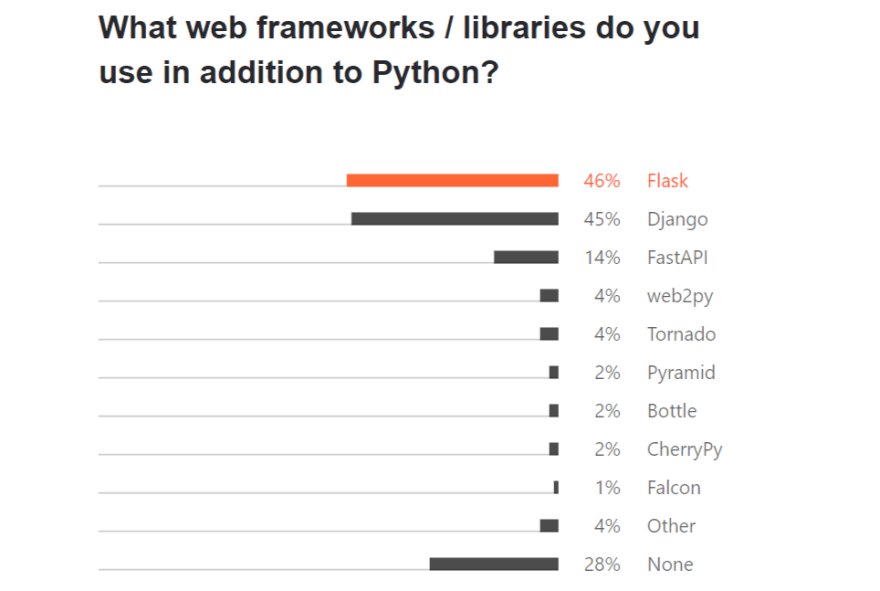
\includegraphics[scale=0.4]{hg2dcbj3lvu2jbjjtdd4}
\caption{\footnotesize{Popularity of major Python web frameworks}}
\captionsetup{aboveskip=0pt,font=it}
\end{figure}
\bigskip

\bigskip
\bigskip
\textbf{{\Large Chapter 3.4 Hypothesis and Excepted Results}}

Since we are undertaking the experiment to either solidify or disprove our expected outcome, we have came up with our own hypothesis of the experiment. From the research and literature review we have undertaken, we understand that WebAssembly have a better performance than JavaScript in web browsers, as well as a faster "code-start" time and lower overhead when running on the server-side. Furthermore, it has a strong, technical community to issue updates and patches regularly as well as working on runtime efficiency and overhead reduction. Resulting in the technology getting more widely adopted as time move on. Therefore, we consider WebAssembly to be a serious contender in the future of commercial server-side development. And we except to see a better performance towards the WebAssembly framework in our experiment. We will present our hypothesis in greater details in the upcoming experiments section.